\documentclass[12pt]{article}
\usepackage[a4paper,left=2cm, right=2cm, top=2cm, bottom=2cm]{geometry}
\usepackage{amssymb}
\usepackage{amsmath,mathtools}
\usepackage{relsize}
\usepackage{epsfig,graphicx}
\usepackage{color}
\usepackage{xcolor}
\usepackage{tikz}
\usepackage[authordate16,backend=biber]{biblatex-chicago}
\addbibresource{citation.bib}
\usepackage{color, colortbl}
% \usepackage{subfigure}
\usepackage{hyperref}
\usepackage{algorithm}
\usepackage{algorithmic}
% \usepackage{cite}
\usepackage{amsfonts}
\usepackage{textcomp}
\usepackage{xcolor}
\usepackage{multirow}
\usepackage{authblk}
\usepackage{subcaption}
\usepackage{nameref}
\usepackage{xstring}
\usepackage[labelfont=bf]{caption}
\begin{document}



\begin{figure}[H]
    \centering
    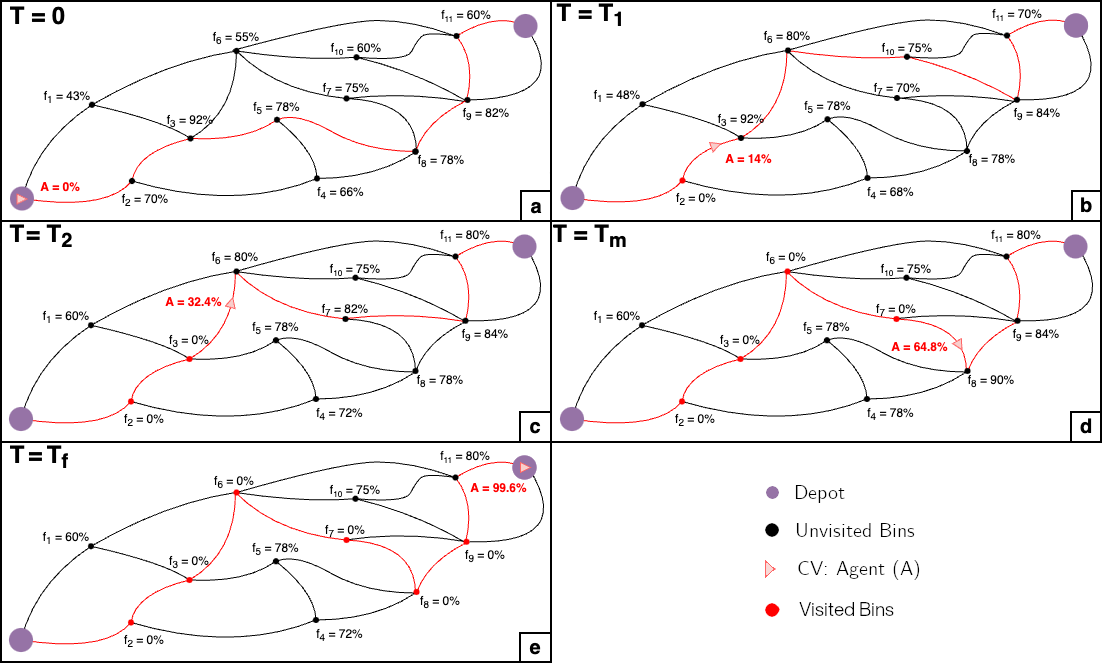
\includegraphics[scale=0.55]{Figure 1.png}
    \caption{General representation of the dynamism of the process}\label{fige}
\end{figure}


\newpage

\begin{figure}[H]
    \centering
    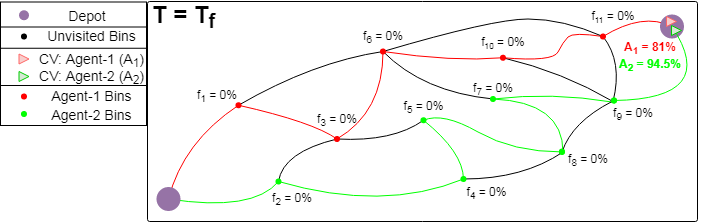
\includegraphics[scale=0.6]{Figure 2.png}
    \caption{General representation of the process for multiple agents}\label{fige2}
\end{figure}

\newpage

\begin{figure}[H]
    \centering
    \includegraphics[scale=0.5]{Figure 3.png}
    \caption{The selected bins and their clusters}\label{figm}
\end{figure}

\newpage
\begin{figure}[H]
    \centering
    \includegraphics[scale=1.35]{Figure 4.png}
    \caption{Analysis of real-time restricted case}\label{figcom}
\end{figure}
\newpage

\begin{figure}[H]
    \centering
    \includegraphics[scale=0.55]{Figure 5.png} % New Image added
    \caption{Realtime Unrestricted}\label{fig2}
\end{figure}


\newpage
\begin{figure}[H]
    \centering
    \includegraphics[scale=0.55]{Figure 6.png} % Image changed here
    \caption{Routes for 3 CV per region as calculated by static optimization}\label{fig4}
\end{figure}
\newpage
\begin{figure}[H]
    \centering
    \includegraphics[scale=0.55]{Figure 7.png} % Image changed here
    \caption{Routes for 3 CV per region as calculated by real-time optimization}\label{fig5}
\end{figure}


\newpage

\begin{figure}[H]
	\centering
	\includegraphics[scale=0.92]{Figure 8.png}\label{ABCD}
	\caption{Detailed static vs dynamic performance analysis}\label{figcg1}
\end{figure}

\end{document}